\chapter{Máquina de aprendizado}

Como no Twitter as publicações criadas por usuários dizem respeito aos mais variados temas, uma busca simples por uma palavra-chave pode retornar publicações relacionadas à ela nos mais variados contextos.

É necessário que o detector de eventos através do Twitter seja capaz de informar se determinada publicação está relacionada ao evento em questão ou não. Essa informação, porém, não pode ser extraída a partir de única publicação. Não é possível, pois, não existem regras para a criação de publicações, e elas podem ser encontradas com as mais variadas combinações e sentidos, portanto não existindo a possibilidade da criação de um conjunto de regras que classifiquem automaticamente as mesmas.

Para resolver esse problema, o modelo implementado utiliza o método de aprendizado supervisionado SVM, para classificar as publicações entre relevantes ou não para a análise.

Os métodos de aprendizado supervisionado são técnicas de aprendizado de máquina que se baseiam na representação do conhecimento do ambiente a partir de um professor. Eles são capazes de aprender as características de um ambiente, ao receberem essa informação de uma fonte externa. Ou seja, o SVM é capaz de receber o conhecimento de quais publicações são relevantes para a análise (dizem respeito à manifestações reais) e quais não são. 

O conhecimento é passado para o algoritmo através da classificação manual de um conjunto de publicacões de amostra. Ao fazer isso, as informações do ambiente estão sendo representadas, o SVM recebe as informações e, através do princípio de indução, consegue utilizar esse conhecimento para fazer induções futuras sobre outros dados.

O SVM possui o conhecimento de cada entrada de informação e baseia-se na semelhança entre os mesmos para determinar as suas classes. Ou seja, ao classificar um conjunto inicial de dados, o que está sendo transferido são os padrões de comportamento pertencente a cada classe. O algoritmo, então, que consegue determinar o comportamento de cada classe e classificar futuros dados baseados nessa semelhança.

O princípio de indução, porém, muitas vezes deve ser sensível à erros de classificação, em casos que o conhecimento total do ambiente não pode ser transferido para o ambiente amostral, devido à quantidade de regras ser infinita ou desconhecida. Em um ambiente hipotético binário, por exemplo, aonde se o dado contém ``X'', a classe é ``1'', e se não contém a classe é ``0'', o algoritmo não precisa ser sensível à erros. Mas ao lidar com documentos de texto, por exemplo, as regras de linguagem são mais complexas do que isso. A quantidade de palavras existentes são muitas e elas podem ser encontradas em ordens diferentes, garantindo que o número de possibilidades sejam infinitas ou impossíveis de serem tratadas. Nesse caso, o algoritmo mesmo que não acerte 100\% das classificações, pode chegar à um número de acertos muito próximo disso, mesmo que as regras não sejam todas definidas. 

Para o modelo implementado, como o total de regras é desconhecido, é necessária um conjunto de publicações que seja relevante para representar o conhecimento ao algoritmo. Se o conjunto for reduzido demais, as regras mais importantes podem não ser representadas e o algoritmo irá falhar ao classificar futuros dados. Porém, se o conjunto for extenso demais, o trabalho em classificá-las manualmente será demasiado. É preciso achar um número de publicações que consiga generalizar os dados e que ainda faça sentido a implementação do algoritmo.

Após a criação dos dados de exemplo, o classificador pode ou não passar pela fase de testes, aonde sua taxa de acertos é analisada e verificada se atende às expectativas. No detector proposto, é criada uma nova base de publicações, que são classificadas manualmente, porém o conhecimento dessa nova base não é transferido para o SVM. O algoritmo é então executado e as saídas são analisadas e comparadas com a classificação manual. Para chegar à um resultado satisfatório, o algoritmo é executado sucessivas vezes. De acordo com a sua taxa de acerto, a base de conhecimento é alterada e o parâmetro de custo do algoritmo é ajustado.

Com o conhecimento devidamente representado, o SVM está apto a classificar futuras ocorrências. O SVM é então executado com a base de publicações obtidas do Twitter, e as ocorrências positivas são utilizadas para serem agrupadas por horário e os eventos serem detectados.

\section{Máquina de vetores de suporte (SVM)}

As \textit{máquinas de vetores de suporte} são um conjunto de métodos desenvolvido por Vladimir Vapnik nos anos 90 que, desde a sua criação, superou em performance muitos outros algoritmos existentes, tornando-os a principal linha de pesquisa na área de aprendizado de máquina nos últimos anos \cite{Grigorik2008}. 

Segundo \citeonline{Joachims1998}, o SVM é adequado para a classificação de texto por possuir proteção contra o ajuste demasiado ao conjunto de dados analisados e utilizar \textit{funções de kernel}, que são capazes de lidar com dados de altíssimas dimensões sem a perda de performance.

O SVM é um \textit{problema de otimização}, que recebe como entrada os vetores de características dos dados e os distribui por uma superfície n-dimensional, para que se possa realizar operações com os mesmos. A Figura 4.1 representa um espaço vetorial de documentos de 3 dimensões.

\begin{figure}[htpb]
	\begin{center}
		\includegraphics[width=0.6\textwidth]{figuras/representacao-doc.pdf}
		\caption{Representação vetorial do espaço de documentos. \cite{Salton1975}}
	\end{center}
\end{figure}

Para descobrir quais vetores pertencem à quais classes, o SVM tenta achar um plano, de dimensão n-1, que separa os vetores com a maior margem possível. O algoritmo parte do princípio que existe uma diferença fundamental que separa as duas classes e cria a separação espacial entre elas. O método deduz que, após a criação do plano, os vetores de um lado do plano fazem parte de uma classe e os do outro lado de outra classe, o que na prática se mostra funcionar \cite{Grigorik2008}. 

\subsection{Problema de otimização}

Dado o conjunto de $n$ dados de treinamento:

\begin{equation*}
D = \begin{Bmatrix}
({x}_{i}, {y}_{i}) \mid {x}_{i} \in {R}^{d}, {y}_{i} \in \{-1,1\} 
\end{Bmatrix}
\begin{matrix}
n \\ 
i = 1
\end{matrix}
\end{equation*}

aonde cada ponto ${x}_{i}$ é um vetor de características d-dimensional de números reais e ${y}_{i}$ a classe em que o vetor pertence e possui o valor 1 ou -1. Deseja-se encontrar o plano $p$ que divide o os pontos que possuem ${y}_{i} = 1$ dos que possuem ${y}_{i} = -1$. Cada plano pode ser, então, definido em função de $x$.

\begin{equation*}
wx - b = 0,
\end{equation*}

ou de forma simplificada:

\begin{equation*}
{w}^{T}x + b = 0.
\end{equation*}

Sendo ${w}$ o vetor normal do plano $p$ e $b$ o deslocamento em relação a origem. Para ilustrar o SVM, na Figura 4.2 são representados algumas retas possíveis para dividir duas classes de dados no ${R}^{2}$. Para dados no ${R}^{3}$, o divisor dos dados é um plano bidimensional, para dados no ${R}^{n}$, o divisor dos dados é um hiperplano de dimensão $n-1$.

\begin{figure}[htpb]
	\begin{center}
		\includegraphics[width=0.6\textwidth]{figuras/svm-plans.pdf}
		\caption{Planos possíveis para divisão de duas classes de dados.}
	\end{center}
\end{figure}

Se os dados de treinamento são linearmente separáveis, é possível encontrar dois planos que os separam sem existir nenhum ponto entre eles. Como ${y}_{i}$ possui valor 1 ou -1, os planos que se encontram exatamente no limiar dos pontos são definidos pelas equações (como ilustrado na Figura 4.3):

\begin{equation*}
{w}^{T}x + b = 1,
\end{equation*}

e

\begin{equation*}
{w}^{T}x + b = -1.
\end{equation*}

\begin{figure}[htpb]
	\begin{center}
		\includegraphics[width=0.8\textwidth]{figuras/svm-plans-2.pdf}
		\caption{Planos no limiar dos pontos.}
	\end{center}
\end{figure}

Ou seja, a função de classificação pode ser definida como:

\begin{equation*}
  \begin{cases}
	{w}^{T}x + b \geq 1 & \text{ para ${x}_{i}$ da primeira classe }  \\ 
	{w}^{T}x + b \leq -1 & \text{ para ${x}_{i}$ da segunda classe }
	\end{cases}
\end{equation*} 
	
Na forma reduzida:

\begin{equation*}
	{y}_{i}({w}^{T}{x}_{i} + b) \geq 1, \text{para todo } 1 \leq i \leq n
\end{equation*}

Somente os pontos mais próximos, chamados de \textit{vetores de suporte}, influenciam a criação dos planos, ao contrário do filtro de kalman e regressão linear, por exemplo, que utilizam todos os pontos para gerar o modelo. A distância entre os vetores de suporte positivos e negativos delimita a \textit{margem}.

Para calcular a margem, como ${w}^{T}x + b = 0$ e $c({w}^{T}x + b) = 0$ definem o mesmo plano, é possível escolher a normalização de $w$. A normalização é escolhida tal que ${w}^{T}{x}_{+} + b = 1$ e ${w}^{T}{x}_{-} + b = -1$, para os vetores de suporte positivos e negativos. A margem entre os planos pode ser escrita, então, por:

\begin{equation*}
	\frac{w}{||w||}({x}_{+} - {x}_{-}) = \frac{{w}^{t}({x}_{+} - {x}_{-})}{||w||} = \frac{2}{||w||}
\end{equation*}

O problema de otimização do SVM é maximizar a margem $\frac{2}{||w||}$, ou seja, minimizar $||w||$ (como ilustrado na Figura 4.4). Podendo ser descrito, então, como:

\begin{equation*}
\begin{matrix}
\min & ||w|| & \\ 
\text{sujeito à } & {y}_{i}({w}^{T}{x}_{i} + b) \geq 1, & \text{para todo } 1 \leq i \leq n
\end{matrix}
\end{equation*}

\begin{figure}[htpb]
	\begin{center}
		\includegraphics[width=0.7\textwidth]{figuras/svm-regions-2.pdf}
		\caption{Margem entre os planos.}
	\end{center}
\end{figure}

Nesse método, chamado de \textit{SVM de Margem Rígida}, o modelo se enquadra exatamente aos dados de exemplo. Mas podem existir casos aonde os dados são linearmente separáveis, porém existe uma margem muito pequena entre os vetores de suporte. Nesse caso, o exemplo tentará dividir as classes encontrando como plano ideal um de margem muito pequena, mas talvez um plano de margem maior e que ignore certos pontos seja uma solução mais satisfatória, como ilustrado na Figura 4.5.

\begin{figure}[htpb]
	\begin{center}
		\includegraphics[width=0.7\textwidth]{figuras/svm-soft-margin.pdf}
		\caption{Plano de maior margem que ignorando certos pontos.}
	\end{center}
\end{figure}

O método SVM que permite erros de classificação é chamado de SVM de Margem Suave (\textit{Soft Margin SVM}).

\subsection*{SVM de Margem Suave}

O método Margem Suave introduz a variável de folga ($\xi$):

\begin{equation}
\begin{matrix}
\min & ||w|| + C \sum {\xi}_{i} & \\ 
\text{sujeito à } & {y}_{i}({w}^{T}{x}_{i} + b) \geq 1 - {\xi}_{i}, & \text{para todo } 1 \leq i \leq n
\end{matrix}
\end{equation}

\begin{itemize}
	\item Se $\xi = 0$, o ponto está na margem ou após
	\item Se $0 < \xi \leq 1$, o ponto está entre a margem e o lado correto (violação de margem)
	\item Se $\xi \geq 1$, o ponto está do lado errado, como indicado na Figura 4.6.
\end{itemize}

\begin{figure}[htpb]
	\begin{center}
		\includegraphics[width=0.8\textwidth]{figuras/svm-epsilons.pdf}
		\caption{Valores para $\xi$.}
	\end{center}
\end{figure}

O algoritmo inclui também a constante de custo ($C$), que representa qual o custo de cada erro de classificação e deve ajustado de acordo com o conjunto de dados de exemplo através de validação. 

\begin{itemize}
	\item Se o valor de $C$ é baixo, as restrições são ignoradas facilmente: maior margem.
	\item Se o valor de $C$ é alto, as restrições são mais difíceis de ser ignoradas: menor margem.
	\item Se $C = \propto$, nenhuma restrição é ignorada: \textit{Margem Rígida}.
\end{itemize}

O ajuste correto de $C$ é importante pois aumenta ou diminui a performance do classificador referente ao conjunto de dados da representação de conhecimento. É preciso achar um valor para $C$ que reflita a base de exemplos, para maximizar os acertos do classificador. Se a representação de conhecimento está bem generalizada, é possível que se possa escolher um valor alto para $C$, pois os erros esperados serão poucos. Se está mal generalizada, talvez $C$ com um baixo seja mais adequado, pois espera-se mais erros e mais versatilidade por conta do classificador.

É possível que, mesmo com margem suave, o SVM não consiga classificar os dados de forma linear. Caso isso ocorra, e necessária a aplicação de \textit{funções de kernel}, que são funções que aplicam transformações nos dados para que sejam mais facilmente classificáveis.

\subsection*{Funções de Kernel}

As \textit{funções de kernel} são uma classe de algoritmos utilizados para encontrar e estudar tipos de relações em conjuntos de dados. Atualmente, elas tem recebido grande atenção, particularmente devido à popularidade do SVM. Como pode ser observado nos trabalhos de \citeonline{Ali2005}, \citeonline{Ozer2013}, \citeonline{Megri2014}, entre outros.

As funções de kernel mapeam os dados em um espaço de maior dimensão, com o intuito de que esse espaço seja mais facilmente classificado. A Figura 4.8 representa um espaço de duas dimensões mapeados para um espaço de três dimensões.

\begin{figure}[htpb]
	\begin{center}
		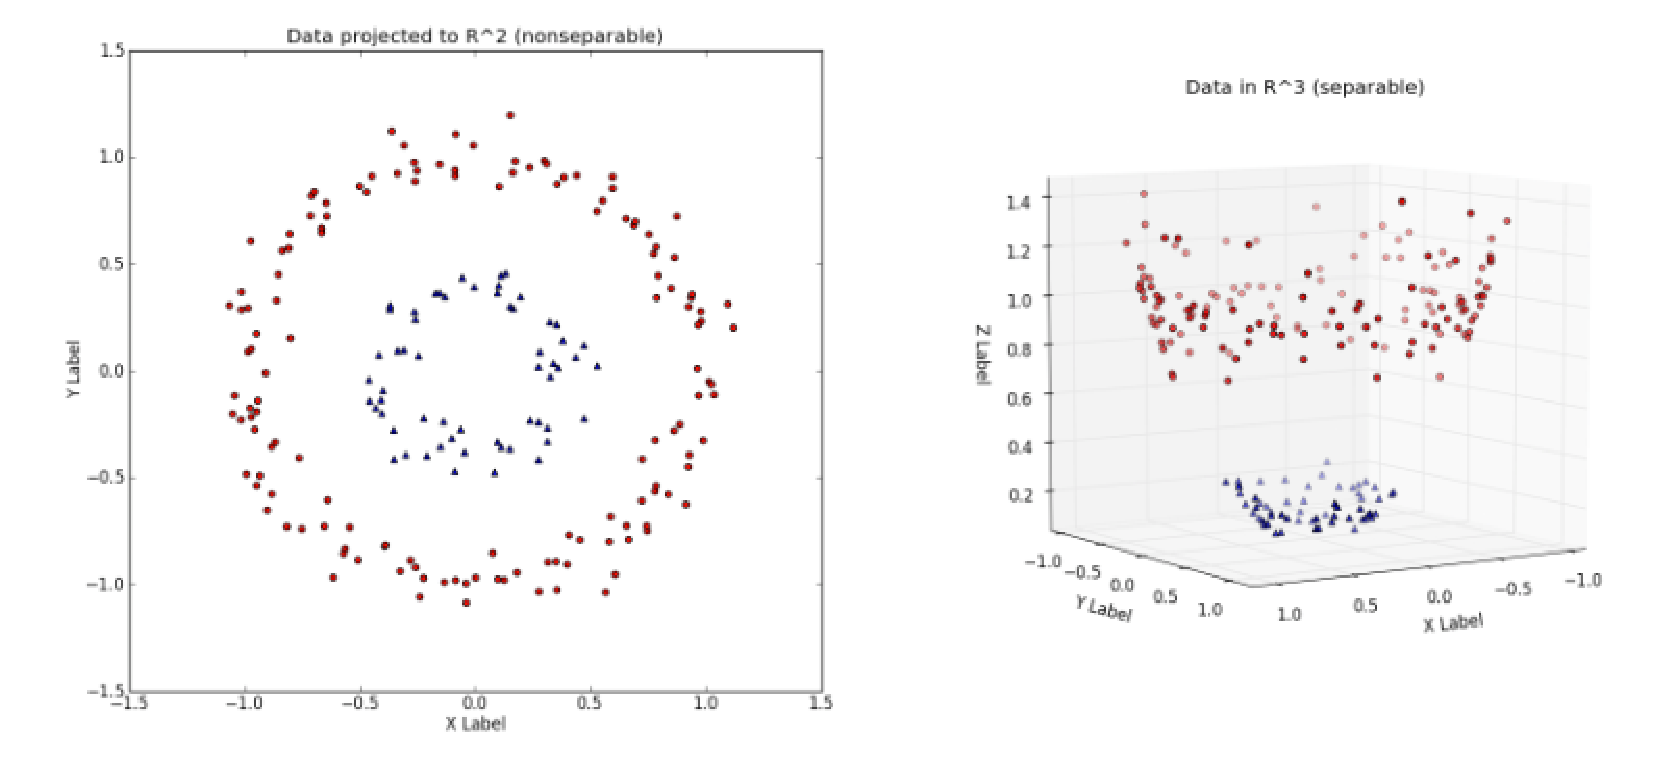
\includegraphics[width=0.9\textwidth]{figuras/svm-kernel.eps}
		\caption{Um conjunto de dados no ${R}^{2}$ (não separáveis) transormados para ${R}^{3}$ (separáveis) pela função de kernel $[{x}_{1}, {x}_{2}] = [{x}_{1}, {x}_{2}, {x_1}^{2} + {x_2}^{2}]$ \cite{Kim2013}.}
	\end{center}
\end{figure}

Os kernels são utilizados em problemas que não precisam operar com os vetores no espaço de maior dimensão, como é o caso do SVM. As funções calculam o produto escalar dos dois vetores no espaço de maior dimensão, sem explicitamente transformá-los para esse espaço. Esse fato possibilita que os kernels operem em dados sem calcularem suas coordenadas, podendo operar em espaços de qualquer dimensão (infinitas) e implícitos.

Existe uma grande variedade de kernels disponíveis. Segundo \citeonline{Grigorik2008}, o \textit{kernel linear} é geralmente bom para 99\% dos casos, mas a escolha da função de kernel adequada pode melhorar a performance do classificador.

\section{Representação do conhecimento}

O SVM é um classificador de aprendizado supervisionado, ou seja, é capaz de aprender à dividir um conjunto de dados em classes distintas. O método aprende a realizar a classificação através da \textit{representação do conhecimento} desse conjunto de dados.

Na representação do conhecimento, algumas ou todas características do conjunto de dados são previamente transferidas para o classificador. Esse conhecimento é transferido pela figura de um professor, que as informa ao classificador com o intuito que ele possa fazer induções futuras a partir dessas informações.

A fase em que se informa propriamente conhecimento ao classificador é denominada de \textit{treinamento}, aonde serão passados tipicamente os vetores de características ${x_i}$ de dados de exemplo e suas respectivas classes ${y_i}$ ao SVM.

Após a fase de treinamento, o SVM pode passar, ou não, pela fase de testes. Aonde o classificador é executado para testar se suas saídas estão satisfatórias, se sua taxa de acerto é aceitável para o modelo em questão. Nesse caso, os vetores de características ${x_i}$ são inseridos, porém as suas classes ${y_i}$ são obtidas pelas saídas do SVM.

\subsection{Treinamento}

Para o treinamento do SVM, o conjunto de dados para ${x_i}$ e ${y_i}$ é criado. Para o modelo implementado, ${x_i}$ serão os vetores de características das publicações, e ${y_i}$ as suas respectivas classes. Cada classe de publicação ${y_i}$ possuirá valor ``1'' caso seja uma ocorrência real de manifestação e ``-1'' caso não seja. Como indicado na Figura 4.9. 

\begin{figure}[htpb]
	\begin{center}
		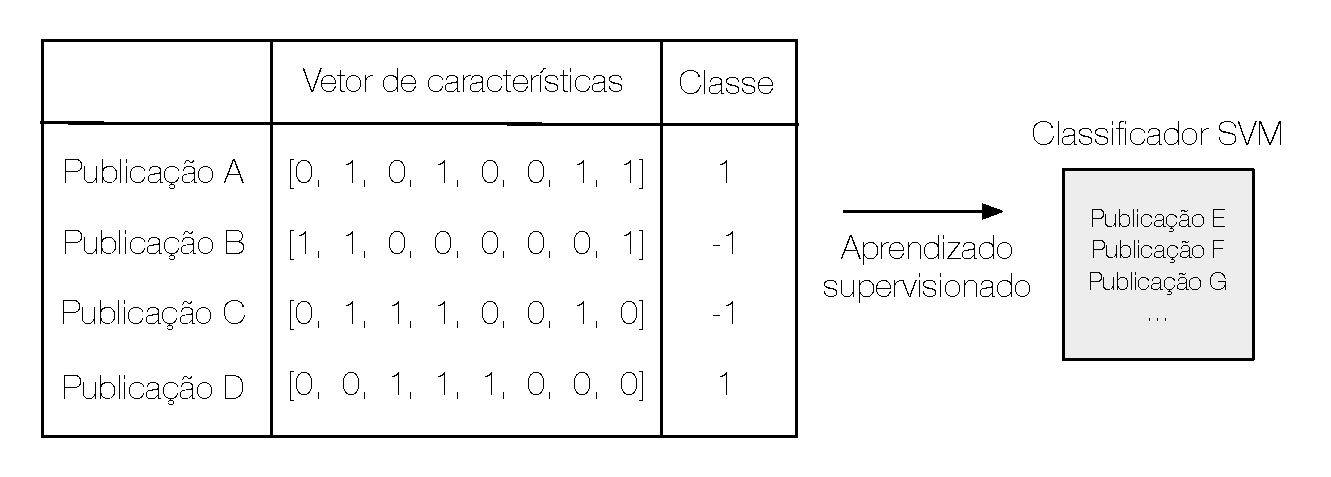
\includegraphics[width=0.8\textwidth]{figuras/inducao-aprendizado-supervisionado.eps}
		\caption{Treino do SVM.}
	\end{center}
\end{figure}

As publicações que indicam a ocorrência de um evento de manifestação podem se apresentar de várias formas, mas devem possuir pelo menos uma característica: representam uma manifestação real, com local e horário, que ocorre no momento da publicação.

As publicações negativas também se apresentam de várias maneiras, não importando muito suas características, podendo ser publicações que mencionam uma manifestação que já aconteceu, que citam uma manifestação que acontecerá no futuro, que utilizam a palavra-chave em outro contexto, etc. 

Um exemplo de publicação positiva é a frase ``manifestação agora na rua Rio Branco'', que informa corretamente o acontecimento de um evento de manifestação e o seu local. Um exemplo negativo é a frase ``odeio manifestação'', que apenas menciona a palavra, não se referindo à um evento. A Tabela 3 apresenta alguns outros exemplos.

\begin{table}[ht]
	\caption{Publicações de treino.}
	\centering
	\begin{tabular}{| p{7cm} | p{7cm} |}
		\hline
		\textbf{Positiva (1)} & \textbf{Negativa (-1)} \\ [0.5ex] \hline \hline
    ``manifestação agora na rua Rio Branco.'' & ``odeio manifestação'' \\ \hline
    ``grupo bloqueia avenidas de SP em manifestação'' & ``vamos fazer uma manifestação'' \\ \hline
    ``ativias param rua de BH em manifestação'' & ``ontem teve manifestação aqui na minha cidade'' \\ \hline
    ``MANIFESTAÇÃO: estudantes bloqueiam BR-101'' & ``sabe se está tendo manifestação?'' \\
    ... & ... \\ [1ex]
		\hline
	\end{tabular}
	\label{table:nonlin}
\end{table}

Para representar esse conhecimento ao SVM, uma base de publicações, as \textit{publicações de treino}, é selecionada a partir do total de publicações obtidas pelo Twitter para o mês de Agosto. As publicações de treino são lidas e classificadas manualmente. Espera-se, então, que ao alimentar o SVM com esse conhecimento, o método consiga aprender os padrões pertencentes à cada classe de publicação e consiga induzir as classes de ocorrências futuras.

Com ${x_i}$ e ${y_i}$ conhecidos, o problema de otimização da Equação 4.1 pode ser resolvido de diversas maneiras, uma delas sendo a \textit{programação quadrática}. O método encontra $w$ e $b$, a partir dos $n$ dados conhecidos de $x$ e $y$. Nesse caso, as publicações de treino e suas respectivas classes.

Com $w$ e $b$ encontrados, o SVM pode ser testado e visto se com os $x$ e $y$ informados, foi suficiente para que ele possa realizar classificações futuras com uma taxa de acerto aceitável.

\subsection{Teste}

Para determinar se a representação do conhecimento é suficiente para o SVM classificar futuras ocorrências, ele é testado em um conjunto de \textit{publicações de teste}. Cada publicação é classificada manualmente, porém a informação não é inserida no classificador. O SVM é então executado e as classificações geradas são comparadas com as classificações manuais.

Como $w$ e $b$ já são conhecidos, a classe $y_i$ do vetor de características $x_i$ de cada publicação pode ser determinada pela seguinte expressão:

\begin{equation}
{y}_{i} = {w}^{T}{x}_{i} + b
\end{equation}

Caso $w$ e $b$ foram gerados satisfatoriamente na fase de treino, as saídas para $y_i$ serão, na maioria das vezes, as classes corretas das publicações.

Caso o classificador não apresente resultados satisfatórios, é possível que o conhecimento não esteja devidamente representado na base de treino e $w$ e $b$ estejam com valores divergentes, ou ainda que o parâmetro $C$ esteja mal ajustado.

A mudança mais fácil de ser feita, nesses casos, é o ajuste do parâmetro $C$. O mesmo deve ser ajustado de acordo com a a base de conhecimento. Se a base estiver bem generalizada, é possível escolher um valor para $C$ mais alto, pois espera-se que o classificador erre pouco. Caso a base não esteja bem generalizada, talvez seja mais adequado escolher $C$ mais baixo, pois ele irá permitir mais versatilidade de adequamento aos dados, porém também permitirá que mais erros ocorram. 

No modelo implementado, o parâmetros $C$ é ajustado através de sucessivos testes, de acordo com a taxa de acerto do classificador. Para implementações com mais parâmetros ou que não seja possível o ajuste manual de $C$, talvez seja necessário a utilização de ferramentas que otimizam múltiplos parâmetros de forma automatizada, como proposto por \citeonline{Chapelle2002}.

Caso o seu ajuste não impacte em mudanças nos acertos das classificações, é possível que o conhecimento não esteja devidamente representado. Se a base de treino for insuficiente, é possível que esteja com poucos exemplos das possibilidades do ambiente ou com exemplos que não reflitam essas possibilidades. O primeiro caso resolve-se inserindo mais exemplos na base. O segundo, troncando os exemplos pelos que melhor representam o ambiente.

Após os devidos ajustes, o SVM precisa ser executado novamente e as saídas novamente comparadas. Para tornar os testes viáveis, o conjunto de dados de teste precisa ser enxuto o suficiente para ser comparado manualmente, porém não muito reduzido para ainda ser relevante. 